% !TeX spellcheck = it_IT
\newpage
\section{Diagrammi di sequenza}
\begin{wrapfigure}[10]{r}{5cm}
	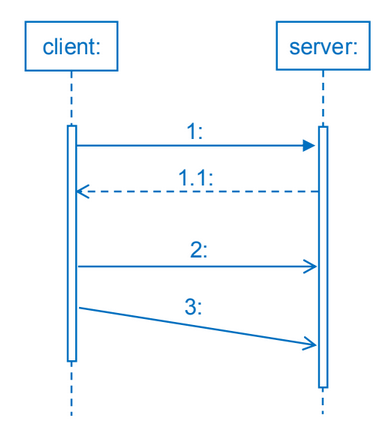
\includegraphics[width=5cm]{diagseq}
\end{wrapfigure}
I diagrammi di sequenza descrivono le \textbf{interazioni} tra oggetti riorganizzandole in una sequenza temporale. Nella fase di \textit{analisi} dei casi d'uso formalizzano la sequenza principale  degli eventi mentre in fase di \textit{progettazione} illustrano come l'architettura realizza i requisiti.\\

In UML per ogni partecipante viene disegnata una \textbf{linea di vita} che può essere tratteggiata quando l'oggetto è inattivo e doppia-continua quando è attivo. Per rappresentare le \textbf{interazioni} vengono usate frecce, che possono essere:
\begin{itemize}
	\item \textbf{Sincrone}
	\item \textbf{Ritorno}
	\item \textbf{Asincrone}
	\item Asincrone con \textbf{consumo di tempo}
\end{itemize}

\subsection{Etichette}
È possibile mettere etichette ai messaggi:
\begin{itemize}
	\item $n$ è il numero del messaggio nella sequenza
	\item \textbf{attr} è l'attributo a cui assegnare il valore restituito
	\item \textbf{name} identifica e descrive il messaggio
	\item \textbf{arg} sono i parametri
	\item \textbf{value} rappresenta il valore restituito
\end{itemize}
\begin{center}
	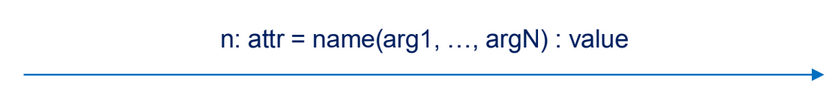
\includegraphics[scale=.4]{etichette}
\end{center}

\subsection{Creazione e distruzione}
Un oggetto può crearne o eliminarne un altro attraverso lo scambio di messaggi.
\begin{center}
	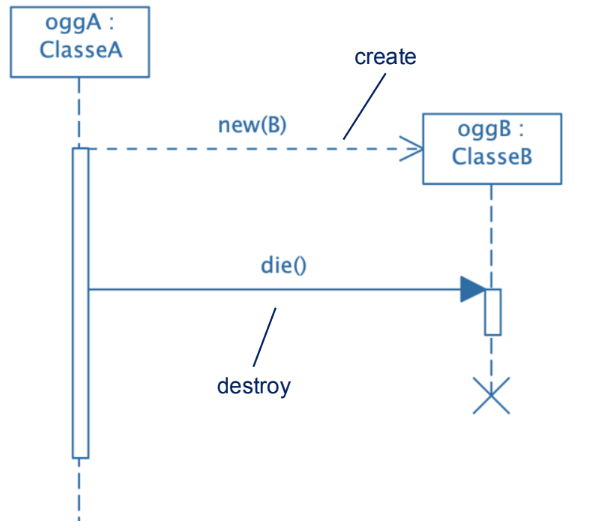
\includegraphics[scale=0.4]{creazdist}
\end{center}

\subsection{Frame}
\subsubsection{Condizionale}
È identificato dalla parola \textbf{alt}. I subframe possono essere etichettati con guardie:
\begin{itemize}
	\item Se non c'è la guardia, è \textit{true}
	\item Se ci sono più guardie vere è una situazione di non determinismo
	\item Se ci sono tutte le guardie false, si salta il frame
\end{itemize}
\begin{center}
	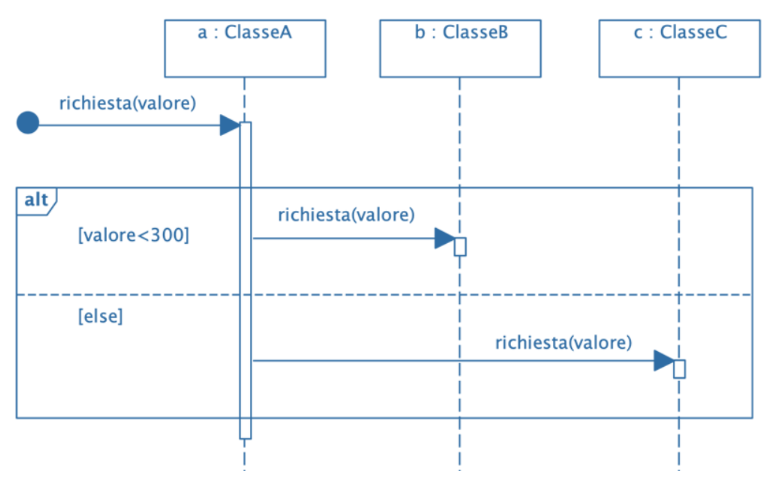
\includegraphics[scale=.3]{condiz}
\end{center}

\subsubsection{Opzionale}
Il frame opzionale è identificato dalla parola chiave \textbf{opt} e le interazioni sono eseguite solo se la guardia è vera, altrimenti il frame viene saltato.
\begin{center}
	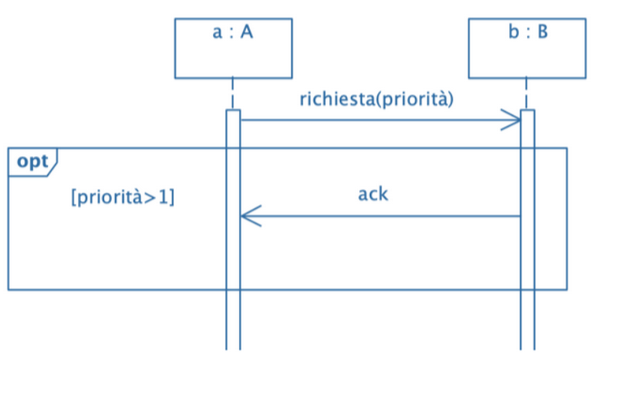
\includegraphics[scale=.3]{opz}
\end{center}

\subsubsection{Iterativo}
Questo frame ripete il suo contenuto da \textit{min} a \textit{max}, \textbf{loop(min, max)} e finché la \textbf{condizione} è vera. Quindi le implementazioni dei classici cicli sono:
\begin{itemize}
	\item \textbf{while}: loop(0,*)[guardia] e loop[guardia]
	\item \textbf{do-while}: loop(1,*)[guardia]
	\item \textbf{for}: loop(n,n) e loop(n)
\end{itemize}
\begin{center}
	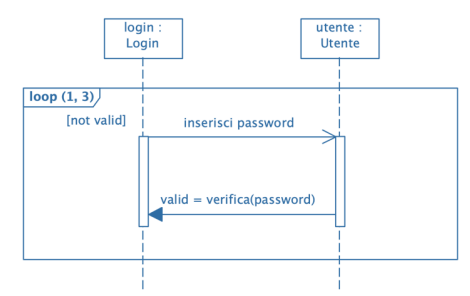
\includegraphics[scale=.4]{cicli}
\end{center}

\subsubsection{Parallelo}
Identificato da \textbf{par}, indica che le interazioni nei sotto-frammenti sono eseguite in parallelo con una semantica ad interleaving.

\begin{center}
	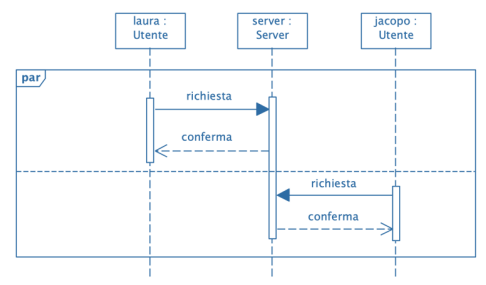
\includegraphics[scale=.5]{parall}
\end{center}

\subsection{Inclusione}
È possibile includere un'interazione definita altrove tramite \textbf{ref}.
\begin{center}
	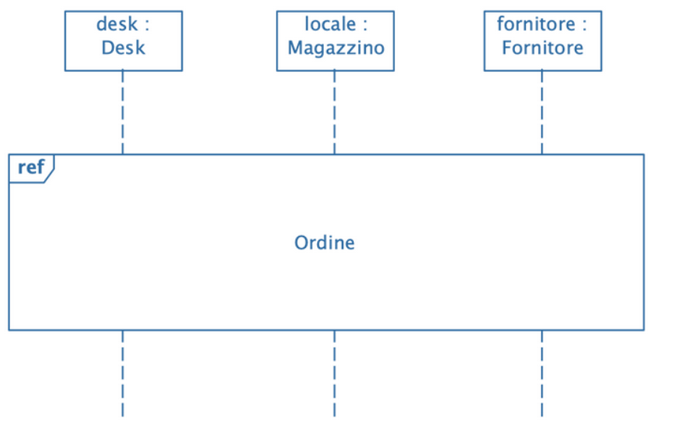
\includegraphics[scale=.4]{ref}
\end{center}

\subsection{Gate}
Un gate è un punto di ingresso o di uscita sul bordo di un diagramma o di un frame. Consente la spedizione e la ricezione di messaggi ed è identificato da un nome.
\begin{center}
	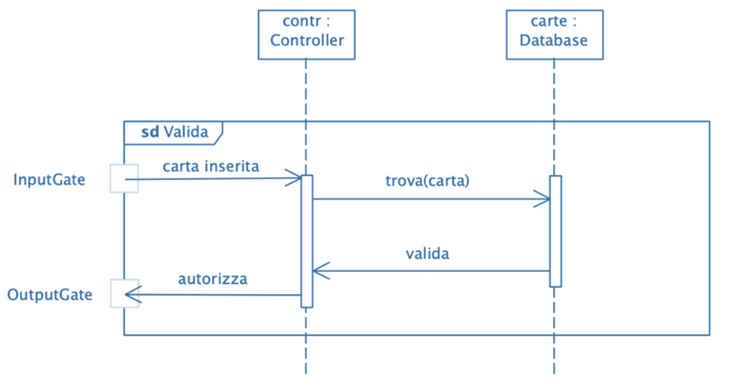
\includegraphics[scale=.4]{gate}
\end{center}

\subsection{Vincoli di durata}
Sono espressi tra parentesi graffe e consentono di specificare:
\begin{itemize}
	\item \textbf{quando} avviene un evento, tramite \textbf{at}(orario) o \textbf{now}
	\item \textbf{quanto} tempo tra due eventi, che può essere un numero effettivo o un range (min, max)
\end{itemize}
\begin{center}
	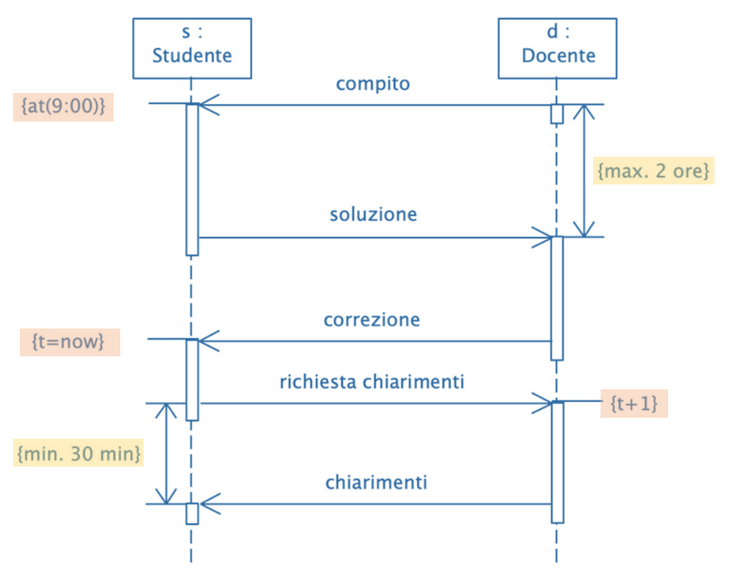
\includegraphics[scale=.4]{vincoli}
\end{center}